\section{تحسين الاستجابة باستخدام التوقع المسبق (\textenglish{Feedforward Control})}
\label{sec:feedforward_control}

تعتمد هيكلية التحكم بالتغذية الراجعة (\textenglish{Feedback Control}) بشكل أساسي على وجود خطأ دائم (\textenglish{Error}) لتوليد إشارة التحكم. هذا يعني أن النظام سيُعاني دائماً من تأخير زمني (\textenglish{Lag}) أثناء الفترات العابرة، مثل أوقات التسارع والتباطؤ السريع، مما يقلل من دقة التتبع الديناميكي للمسار.

للتغلب على هذا القصور الجوهري، تُزود أنظمة السيرفو الحديثة بمسارات تحكم إضافية تُعرف بـ \textbf{التحكم بالتوقع المسبق (\textenglish{Feedforward Control})}. تعتمد هذه الاستراتيجية على حقن إشارات استباقية مباشرة في حلقات التحكم بناءً على المعرفة المسبقة بالمسار المطلوب والنموذج الرياضي للآلة، وذلك لتقليل العبء عن متحكمات الـ \textenglish{PID} وتقليص خطأ التتبع إلى مستويات تقترب من الصفر.

% مخطط يوضح إضافة مسارات التوقع المسبق
\begin{figure}[h!]
    \centering
    \resizebox{\textwidth}{!}{%
    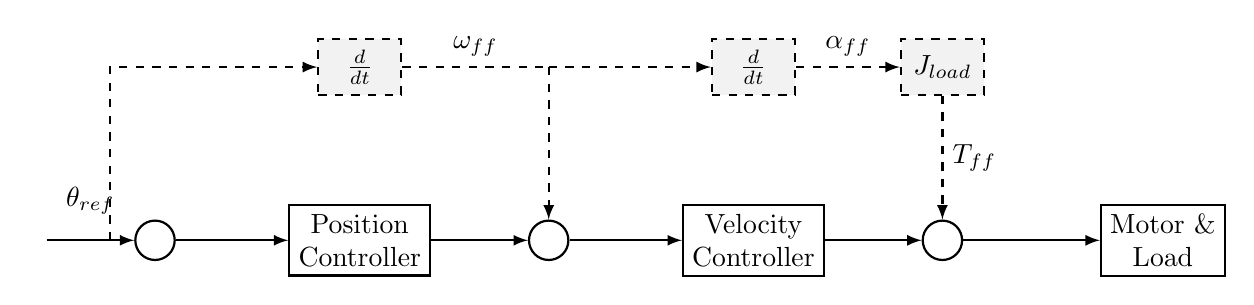
\begin{tikzpicture}[auto, >=latex]
        % تعريف الأنماط
        \tikzstyle{block} = [draw, rectangle, minimum height=2.5em, minimum width=4em, align=center, thick]
        \tikzstyle{ffblock} = [draw, rectangle, minimum height=2em, minimum width=3em, align=center, thick, fill=gray!10, dashed]
        \tikzstyle{sum} = [draw, circle, inner sep=0pt, minimum size=0.5cm, thick]
        
        % المسار الأساسي
        \node (ref_pos) {};
        \node [sum, right of=ref_pos, node distance=1.5cm] (sum_pos) {};
        \node [block, right of=sum_pos, node distance=2.6cm] (ctrl_pos) {\textenglish{Position}\\\textenglish{Controller}};
        
        \node [sum, right of=ctrl_pos, node distance=2.4cm] (sum_vel) {};
        \node [block, right of=sum_vel, node distance=2.6cm] (ctrl_vel) {\textenglish{Velocity}\\\textenglish{Controller}};
        
        \node [sum, right of=ctrl_vel, node distance=2.4cm] (sum_cur) {};
        \node [block, right of=sum_cur, node distance=2.8cm] (plant) {\textenglish{Motor \&}\\\textenglish{Load}};

        % مسارات التوقع (Feedforward) - تمت المحاذاة العمودية لمنع التداخل
        \node [ffblock, above of=ctrl_pos, node distance=2.2cm] (deriv1) {$\frac{d}{dt}$};
        \node [ffblock, above of=ctrl_vel, node distance=2.2cm] (deriv2) {$\frac{d}{dt}$};
        % وضع كتلة القصور الذاتي فوق نقطة الجمع تماماً
        \node [ffblock] at (sum_cur |- deriv2) (inertia) {$J_{load}$};

        % رسم المسارات الأساسية
        \draw [->, thick] (ref_pos) -- node[midway, yshift=0.2cm] {$\theta_{ref}$} (sum_pos);
        \draw [->, thick] (sum_pos) -- (ctrl_pos);
        \draw [->, thick] (ctrl_pos) -- (sum_vel);
        \draw [->, thick] (sum_vel) -- (ctrl_vel);
        \draw [->, thick] (ctrl_vel) -- (sum_cur);
        \draw [->, thick] (sum_cur) -- (plant);
        
        % رسم مسارات التوقع المسبق بدقة هندسية
        \coordinate (takeoff_ff) at ([xshift=0.8cm]ref_pos.east);
        \draw [->, thick, dashed] (takeoff_ff) |- (deriv1.west);
        
        % التفرع الأول (السرعة)
        \draw [thick, dashed] (deriv1.east) -- node[midway, above] {$\omega_{ff}$} (deriv1.east -| sum_vel) coordinate (drop_w);
        \draw [->, thick, dashed] (drop_w) -- (deriv2.west);
        \draw [->, thick, dashed] (drop_w) -- (sum_vel.north);
        
        % التفرع الثاني (التسارع والعزم)
        \draw [->, thick, dashed] (deriv2.east) -- node[midway, above] {$\alpha_{ff}$} (inertia.west);
        \draw [->, thick, dashed] (inertia.south) -- node[midway, right] {$T_{ff}$} (sum_cur.north);

    \end{tikzpicture}%
    }
    \caption[مخطط يوضح حقن إشارات التوقع المسبق (السرعة والعزم) في حلقات التحكم]{\centering مخطط يوضح حقن إشارات التوقع المسبق (السرعة والعزم) في حلقات التحكم الأساسية}
    \label{fig:feedforward}
\end{figure}

تُقسم إشارات التوقع المسبق في أنظمة الحركة إلى نوعين رئيسيين، كما هو موضح في المخطط (\ref{fig:feedforward}):

\subsection{توقع السرعة المسبق (\textenglish{Velocity Feedforward})}
يتم اشتقاق المسار الزاوي المطلوب $\theta_{ref}$ بالنسبة للزمن للحصول على السرعة المرجعية المطلوبة $\omega_{ff}$. تُضاف هذه الإشارة مباشرة إلى مدخل حلقة السرعة (تتجاوز متحكم الموقع). 
\begin{itemize}
    \item \textbf{الفائدة الهندسية:} يقضي هذا المسار بشكل شبه كامل على خطأ التتبع الموضعي (\textenglish{Following Error}) أثناء الحركة بسرعة ثابتة، حيث لا يضطر متحكم الموقع للانتظار حتى يتراكم الخطأ ليُصدر أمر الحركة.
\end{itemize}

\subsection{توقع العزم المسبق (\textenglish{Torque/Acceleration Feedforward})}
لتحقيق تسارع ديناميكي عالٍ دون إرهاق متحكم السرعة، يتم اشتقاق السرعة المرجعية مرة أخرى للحصول على التسارع الزاوي المطلوب $\alpha_{ff}$. بضرب هذا التسارع في عزم القصور الذاتي الكلي للنظام ($J_{load}$)، نحصل على العزم الديناميكي المطلوب $T_{ff}$ بناءً على قانون نيوتن الثاني:
$$T_{ff} = J_{load} \cdot \alpha_{ff}$$
تُضاف هذه الإشارة مباشرة إلى مدخل حلقة التيار.
\begin{itemize}
    \item \textbf{الفائدة الهندسية:} يوفر هذا المسار العزم الإضافي اللازم للتغلب على القصور الذاتي اللحظي أثناء التسارع والتباطؤ، مما يمنع انخفاض سرعة المحرك تحت تأثير الحمل، ويجعل استجابة النظام تبدو وكأنها لا تمتلك قصوراً ذاتياً.
\end{itemize}

\textbf{ملاحظة جوهرية في نظرية التحكم:} على عكس زيادة مكاسب (\textenglish{Gains}) متحكمات الـ \textenglish{PID} التي قد تؤدي إلى عدم استقرار النظام أو الرنين الميكانيكي، فإن إضافة مسارات التوقع المسبق (\textenglish{Feedforward}) \textbf{لا تؤثر إطلاقاً على استقرار حلقة التحكم المغلقة}، لأنها تُحقن من خارج حلقة التغذية الراجعة، مما يجعلها أداة قوية جداً وآمنة لتحسين الأداء الديناميكي.